\documentclass{chi2009}
\usepackage{times}
\usepackage{url}
\usepackage{graphics}
\usepackage{color}
\usepackage[pdftex]{hyperref}
\usepackage[T1]{fontenc}

\hypersetup{%
pdftitle={Vision in Rock Climbing},
pdfauthor={Ryan Drapeau, Sonja Khan, Aaron Nech},
pdfkeywords={computer vision, convolutional neural networks, hourglass CNN},
bookmarksnumbered,
pdfstartview={FitH},
colorlinks,
citecolor=black,
filecolor=black,
linkcolor=black,
urlcolor=black,
breaklinks=true,
}
\newcommand{\comment}[1]{}
\definecolor{Orange}{rgb}{1,0.5,0}
\newcommand{\todo}[1]{\textsf{\textbf{\textcolor{Orange}{[[#1]]}}}}

\pagenumbering{arabic}  % Arabic page numbers for submission.  Remove this line to eliminate page numbers for the camera ready copy

\begin{document}
% to make various LaTeX processors do the right thing with page size
\special{papersize=8.5in,11in}
\setlength{\paperheight}{11in}
\setlength{\paperwidth}{8.5in}
\setlength{\pdfpageheight}{\paperheight}
\setlength{\pdfpagewidth}{\paperwidth}

% use this command to override the default ACM copyright statement
% (e.g. for preprints). Remove for camera ready copy.
\toappear{Submitted to CSE 576 (Spring '16) as the final paper.}

\title{Computer Vision Rock Climbing Using RGB Video}
\numberofauthors{3}
\author{
  \alignauthor Aaron Nech\\
    \affaddr{University of Washington}\\
    \email{necha@\thanks{@cs.washington.edu}}
  \alignauthor Sonja Khan\\
    \affaddr{University of Washington}\\
    \email{sonjak3@\footnotemark[1]}
  \alignauthor Ryan Drapeau\\
    \affaddr{University of Washington}\\
    \email{drapeau@\footnotemark[1]}
}

\maketitle

\begin{abstract}
AJhaksdh
\end{abstract}

\keywords{computer vision, convolutional neural networks}

\section{Introduction}
In recent years, rock climbing has gained more popularity and more traction among people around the world. The logic and problem solving abilities found in bouldering are also common to the core ideas of Computer Science. Therefore, it was inevitable that they would cross paths at some point. In fact, earlier this year Brooklyn Boulders, one of the most popular climbing gyms in the world, released a video showing their new Augmented Reality Climbing project that would be debuting shortly to the public. The project focusses on using a projector to establish ``target'' locations on the wall the must be tapped in quick succession to score the most points, because the goal is to finish the route in as little time as possible. There was earlier work that looked into building a hybrid system with a projector and a rock wall. Both Brooklyn Boulders and Kajastila et. al. built systems that required human input and collaboration throughout the execution in order for the system to be useful. In this paper we will use recent advances in computer vision and convolutional neural networks to automate a system that will assist rock climbers while they are climbing routes.

Our project utilizes a single RGB camera that is mounted on a tripod 5-10 meters away from the rock wall in order to capture the entire wall in its field of view. Brooklyn Boulder's work focuses mainly on using a human at a computer that can detect when holds or targets are touched. A similar system is used in Kajastila's work but with a Kinect camera that can detect one's pose. The main goal of our project is to design a system that is free from these requirements and free from most human interaction. We hope that a system similar to ours could be used to aid rock climbers in improving and refining their skills. Our system could also be used to design games and augmented reality applications when combined with a projector capable of displaying images on a rock wall.

\section{Project Design}

The goal of the project is to provide a robust vision system using only a single RGB camera for rock climbing applications. In our implementation we utilize our vision system to provide interesting post-climb videos showing which handles a climber comes in contact with, and their pose throughout the climbing session. We also aim to have our system run in real-time, enabling interactive experiences.

To accomplish this, we need to decompose such a system into four central components:

\begin{figure*}[t]
  \centering
  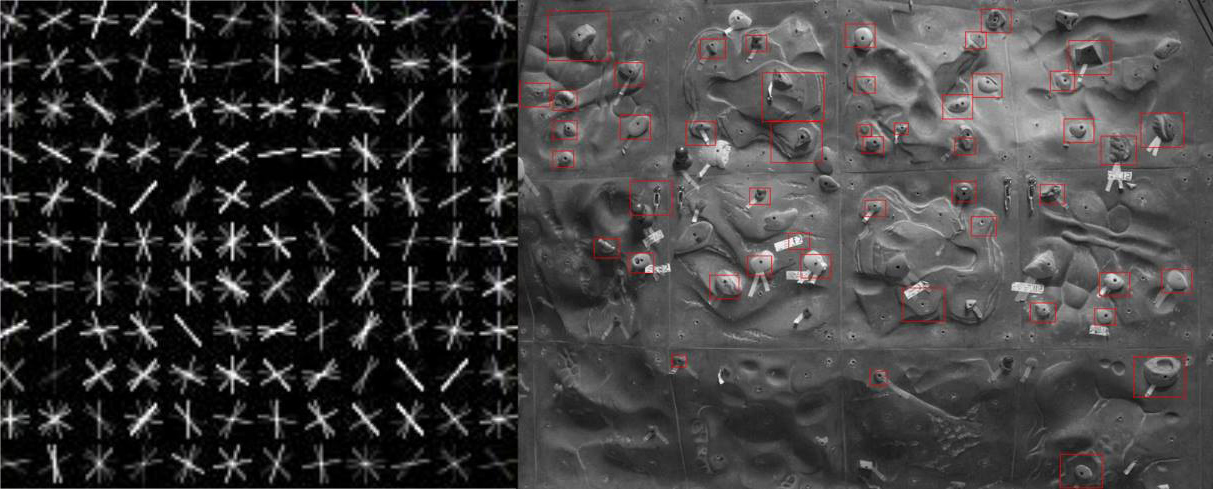
\includegraphics[keepaspectratio, width=\textwidth]{figs/svm_wall.jpeg}
  \caption{Left: \normalfont askd, \textbf{Right:} aslkdjas}
  \label{fig:user}
\end{figure*}

\begin{enumerate}
  \itemsep0em
  \item Physical RGB capture.
  \item Rock climbing handle detection.
  \item Climber isolation from background.
  \item Accurate climber pose estimation (to obtain locations of hands, feet, etc). As well as determine when a handle is being grabbed.
\end{enumerate}

After each sub component is implemented, we can obtain a RGB video camera feed, detect climber handle locations (only once), perform climber isolation, and finally obtain a pose and handle grabbing locations from the isolated climber. Using this information we can construct both interactive and noninteractive applications to enhance rock climbing experience. Finally, to make this all happen we obtained permission from the University of Washington Intramural Activity Center's Crags Climbing Center (Crags) to obtain the raw RGB data necessary for development, as well as test our system.

\section{Implementation}

\subsection{Rock Climbing Handle Detection}

We need only detect rock wall handles once in our video since their location remains fixed in the video frame with respect to time. To detect handles on walls, we found the histogram of oriented gradients (HOG) to be a powerful descriptor, as the main indicator is shape. We extract this descriptor for each handle patch in the rock wall image. We then utilized a Support Vector Machine (SVM) linear classifier to differentiate between handle and non-handle patches, where non-handle patches are selected hard-negatives from the image during the training process. We utilized the open source DLIB machine learning library for it's excellent SVM training framework to accomplish this. Our resulting detector from 100 hand-labeled rock climbing handle examples is shown in the figure.

\subsection{Climber Isolation from Background}

In order to accurately monitor pose and obtain information about the climbing session, we need to know with high certainty where the climber is located during each frame of the video. In this step, we generate a padded bounding box around the human to pass to the pose estimation step, which requires square images where the human is ~75\% of the image.Since the climber is moving, we must update this location with respect to time. Initially we thought of using a regular human detection pipeline, however this is cumbersome and may be error prone. With a simple assumption we can perform much better: since the climbing wall is stationary with respect to the camera, background subtraction is a powerful and real-time option. In particular, we select a reference frame from the beginning of the film that does not have a climber present, we then take the absolute difference between this frame and the current video frame for all time steps forward. Values with a high absolute difference are indicative of the climber (since they are the only object moving in the video). We then threshold this image (using a binary threshold), and dilate all pixels to fill in small holes caused by noise and low differences within the climber. We then find the largest continuous contour in the image and select this as our climber isolation with some padding. The location of each bounding square relative to the full image is stored so we can back project the pose estimation data into the final visualization. For this step and all following steps, we work with downsampled versions of the original video frames in order to increase speed.

\begin{figure*}[t]
  \centering
  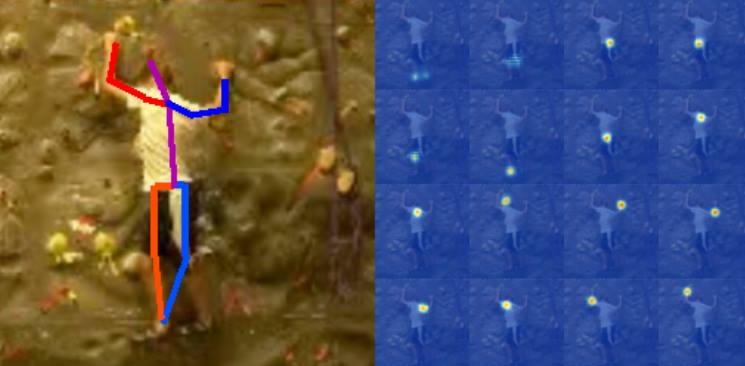
\includegraphics[keepaspectratio, width=\textwidth]{figs/pose.png}
  \caption{Left: \normalfont askd, \textbf{Right:} aslkdjas}
  \label{fig:user}
\end{figure*}

\subsection{Human Pose Estimation}

Once a suitable isolated climber patch is obtained, we are tasked with obtaining an estimate of the climber pose for purposes of detecting which handles the human is interacting with. To accomplish this we utilize a Stacked Hourglass Neural Network to extract human pose from an isolated image patch. Stacked Hourglass Networks are very recent development, and, as of this writing, currently obtain state-of-the-art results on the MPII and FLIC pose estimation benchmarks. The high level idea behind the network is that an hourglass shape that successively compresses the convolved volumes and then expands them via repeated max pooling and upsampling blends information from across the image patch, resulting in more accurate pose estimates. Stacking these hourglass units provides estimates and verification of previous results within the network. The result is a fully end-to-end system which takes a input a human patch, and outputs a heatmap of probabilities for various joint locations. The network is implemented in Torch and has real-time feed-forward speeds when computed on modern GPUs. Estimation of every-nth pose further increases speed.

Our results useing this network for every frame, and although mostly accurate, produces some noise because the network does not have information about previous poses. We therefore made substantial efforts to reduce the noise in this signal. In particular, we consider a temporal 
window of size K of poses. We can calculate the distance of one pose to another via the summed squared difference of each of 16 pose points (one for each body joint). We then can render K frames behind real time, and, using this buffer, compute the median absolute deviation of the window using pose distance as our metric. We then use the median absolute deviation to identify outliers within this window, under the assumption that in fractions of sections, joints should not move much. We also apply averaging in this window to further reduce noise.

Once the pose signal is smoothed, it is the case that some points in the video simply have no pose information (it was not measured, or it was removed as an outlier). In these cases we simply interpolate between known pose locations with a cubic spline curve. The result is a very smooth and accurate pose estimation for the duration of the video.

\subsection{Handle Grab Detection Via Heatmaps}

To detect if the climber is currently holding a handle, we employ a simple decaying heatmap model. In particular we construct an image the same resolution as our downsampled video we are working with. For each time step (frame), we simply add a 2D spatial gaussian to the location of the pose hands and feet (4 gaussians total). We then multiply the entire image by a decay factor (we experimentally chose a decay factor of 0.9). The result is high values where the climber pauses to hold handles, and not significantly high values when the pose is in-transit between handles. We then threshold this map and use a combination of pause locations (determined by our threshold), and our detected handle locations previously determined with our SVM pipeline, to determine if a hold is being grabbed by the climber.

\section{Results}
The results for our handle detection yielded an 80\% recall and 70\% precision. Our climber isolation results are incredibly fast and accurate when applied to various videos taken at the Crags. The raw data noisy for our pose estimation was quite noisy initially, but performs reasonably well after smoothing. We were pleased to find that the neural net accurately picked out occluded joints. This is important because it is quite common in climbing for the body to contort into strange positions and occlude parts of itself. The last step, handle grab detection, relies on the accuracy of the previous steps. In isolation, it performs exactly as expected. 

Combining all of the steps outlined in the Implementation section, we were able to successfully produce a visualization analyzing a climber scaling a bouldering wall. A video of the work can be viewed at https://youtu.be/GkXjrXCHRfc.

\section{Discussion}


\section{Future Work}

There are many different directions for future work that we have considered while working on this project. Using our system in a real-time setting would be an interesting project for future work. We designed and implemented our system so that this would be possible. This was done by utilizing calls to compiled libraries like OpenCV and NumPy since a majority of our project was done in Python. Some of the heavy lifting code was written in C++ to avoid any of the slowdowns that come along with Python. Another exciting direction for this work would be to implement and test a rock climbing game given our framework. Since a climber's pose can be detected as well as the rock holds, this information could be used along with a projector to simulate new routes without having to mark the holds by hand. This gives a lot more flexibility to the route setters in how they design their routes and how exciting those routes could be.

There are also many routes to investigate to improve upon our detection system. One avenue of work would be to incorporate temporal information into the pose estimation step. This would give not only smoother results, but also more accurate results. Another extension to investigate is using a non-stationary camera setup. Currently our system is constrained to the viewing frustrum of one stationary camera, but a climbing route often spans more than this.

\section{Conclusion}
In this paper, we have demonstrated that using computer vision techniques to analyze the movements of a rock climber in a bouldering gym with the input from a single RGB camera is possible. We described our pipeline for determining hold locations, human location, pose estimation, and hold grabbing detection. Finally, we presented our work as a single visualization and discussed many possible extensions of this work.

\section{Acknowledgments}

We would like to thank the University of Washington Crags Climbing Center for allowing us to use their facilities for this project.

\bibliographystyle{abbrv}
\bibliography{references}

\end{document}
